\subsection{Morphological and orthographic features}
\label{sec:feat}

Clark \shortcite{Clark:2003:CDM:1067807.1067817} demonstrates that
using morphological and orthographic features significantly improves
part-of-speech induction with an HMM based model.
Section~\ref{sec:related} describes a number other approaches that
show similar improvements.  This section describes one way to
integrate additional features to the random-substitute model.

In order to accommodate multiple feature types the CODE model needs to
be extended to handle more than two variables.
\cite{globerson2007euclidean} suggest the following likelihood
function:

\begin{eqnarray}
&\ell(\phi,& \psi^{(1)}, \ldots, \psi^{(K)}) = \label{eq:multiscode}\\
&&\sum_k w_k \sum_{x,y^{(k)}} \bar{p}(x,y^{(k)}) \log p(x,y^{(k)}) \nonumber
\end{eqnarray}

\noindent where $Y^{(1)}, \ldots, Y^{(K)}$ are $K$ different variables
whose empirical joint distributions with $X$,
$\bar{p}(x,y^{(1)})\ldots\bar{p}(x,y^{(K)})$, are known.
Eq.~\ref{eq:multiscode} then represents a set of CODE models
$p(x,y^{(k)})$ where each $Y^{(k)}$ has an embedding $\psi_y^{(k)}$
but all models share the same $\phi_x$ embedding.  The weights $w_k$
reflect the relative importance of each $Y^{(k)}$ and all embeddings
are mapped to unit-sphere to fix the $Z^{(k)}$ around a fix value.

We adopt this likelihood function, set all $w_k=1$, let $X$
represent a word, $Y^{(1)}$ represent a random substitute and
$Y^{(2)}, \ldots, Y^{(K)}$ stand for various morphological and
orthographic features of the word.  With this setup, the training
procedure needs to change little: each time a word --
random-substitute pair is sampled, the relevant word -- feature pairs
are also generated and input to the gradient ascent algorithm.

One problem with this setup is, unobserved features misguide the
gradient search algorithm and lead to a suboptimal convergence point.
For example, ``\textbf{car}'' and ``\textbf{red}'' belong to the ``Noun''
and ``Adjective'' clusters, respectivly, and neither of them have a
morphological feature, thus their morphological features are
represented by a null value, ``X''.  However setting the unobserved
features of words from different clusters to ``X'' leads to a false
similarity between these words.  To solve this problem, during the
gradient search we don't perform any pull or push updates on
embeddings if the corresponding $y^{(k)}$ is null\footnote{$x\inX$
  represents a word type therefore it is always observed.}.

The orthographic features we used are similar to the ones in
\cite{bergkirkpatrick-EtAl:2010:NAACLHLT} with small modifications:

\begin{itemize}
\item Initial-Capital: this feature is generated for capitalized words
  with the exception of sentence initial words.
\item Number: this feature is generated when the token starts with a
  digit.
\item Contains-Hyphen: this feature is generated for lowercase words
  with an internal hyphen.
\item Initial-Apostrophe: this feature is generated for tokens that
  start with an apostrophe.
\end{itemize}

We generated morphological features using the unsupervised algorithm
Morfessor \cite{creutz05}.  Morfessor was trained on the WSJ section
of the Penn Treebank using default settings, and a perplexity
threshold of 1.  In our model, a word type consists of two parts: a
stem and a suffix part.  The suffix parts are used as the
morphological feature thus each word type has only one morphological
feature.  We extracted the stem part by concatinating the splits until
including the first ``STM'' labeled split and the suffix part by
concatinating rest of the splits\footnote{The program induced 5575
  suffix types that are present in a total of 19223 word types.}.

%% These suffixes were input to S-CODE as morphological features whenever
%% the associated word types were sampled.  In order to incorporate
%% morphological and orthographic features into
%% S-CODE we modified its input.  For each word -- random-substitute pair
%% generated as in the previous section, we added word -- feature pairs
%% to the input for each morphological and orthographic feature of the
%% word.  Words on average have 0.25 features associated with them.
%% This increased the number of pairs input to S-CODE from 14.1
%% million (12 substitutes per word) to 17.7 million (additional 0.25
%% features on average for each of the 14.1 million words).

Using similar training settings as the previous section, the addition
of morphological and orthographic features increased the many-to-one
score of the random-substitute model to \ftmto\ and V-measure to \ftvm.
Both these results improve the state-of-the-art in part-of-speech
induction significantly as seen in Table~\ref{tab:results}.

\begin{figure*}[ht] \centering
%\vspace*{-10mm}
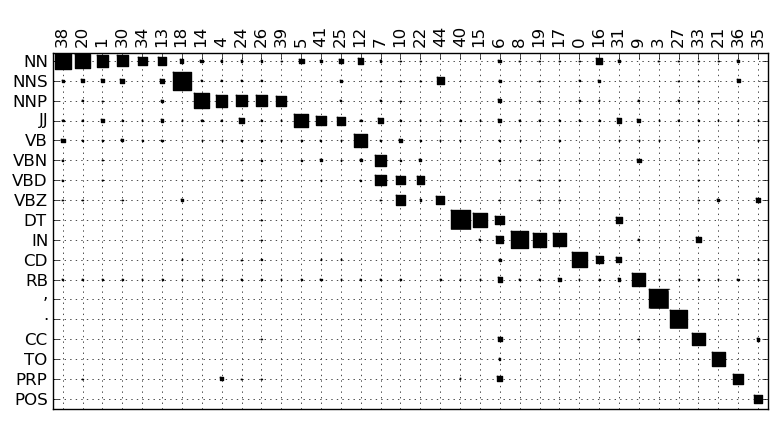
\includegraphics[width=\textwidth]{hinton.png}
%\vspace*{-30mm}
\caption{Hinton diagram comparing most frequent tags and clusters.}
\label{plot-hinton}
\end{figure*}

